\documentclass[12pt]{article}

\usepackage{amsthm}
\usepackage{graphicx}
\usepackage{float}

\begin{document}

\theoremstyle{definition}
\newtheorem{definition}{Definition}[section]

\theoremstyle{remark}
\newtheorem*{remark}{Remark}
\newtheorem{theorem}{Theorem}[section]
\newtheorem{lemma}[theorem]{Lemma}

Let $G$ be a tree with $\Delta \le 4$.\\
\textbf{Question: can $G$ be a unit square graph?} 
Let's call $T_k$ the tree of depth $k$ such that every vertex of $G$ is of degree $4$ except the leaves. \\
$T_0$ and $T_1$ are clearly unit square graphs. However, for $k \ge 2$, it is less obvious. 

\begin{figure}[H]
    \centering
    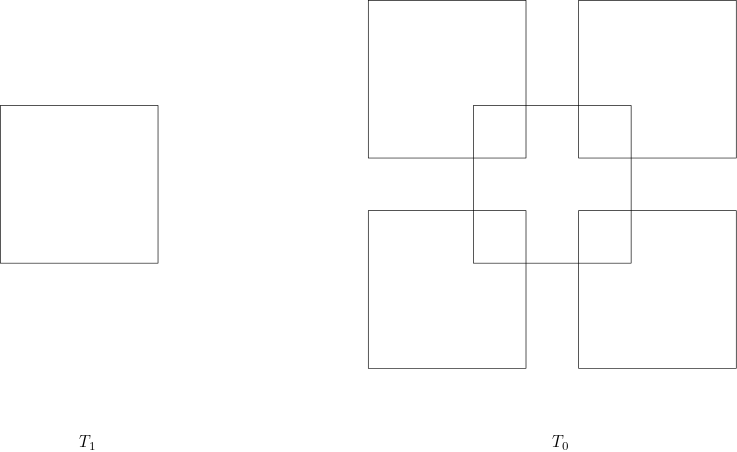
\includegraphics[scale = 0.4]{any_tree.png}
    \caption{$T_0$ and $T_1$ are clearly unit square.}
\end{figure}

Let's observe that: $|T_k| = \sum_{i=0}^{k} 4^i$ meaning the number of vertices increase very fast. However, the maximum euclidean distance between the root vertex and any other vertex of the graph linearly depends on $k$.
For instance, with $k = 5$, $|T_k| = 1365$; but a leaf is at most at distance 5 from the root. Therefore, we ca 

\end{document}